\documentclass[tikz]{standalone}
\usepackage{pgfplots}
%\pgfplotsset{compat=1.8}
\begin{document}
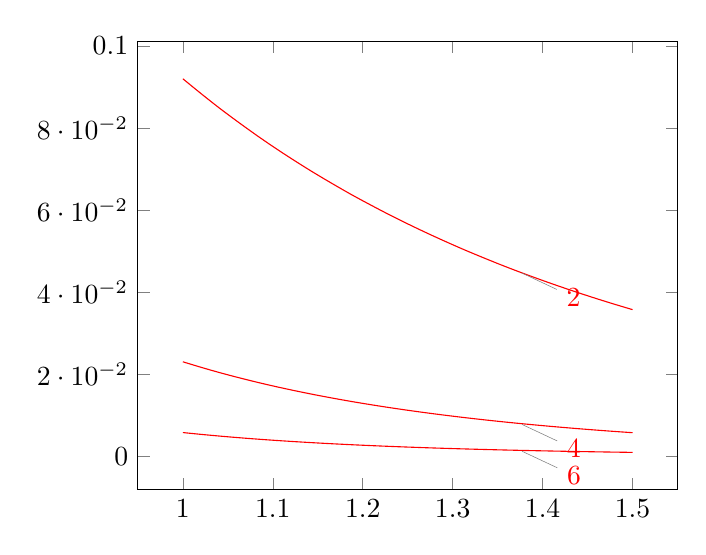
\begin{tikzpicture}[
    declare function={
      %% func(\x)= 10* log2(\x + 1);
      %% g(\x)= 20* log2(\x + 1);
      h0(\x)= exp(-\x) / (\x + 1)^2;
      %% h(\x)= exp(-\x) / (\x + 1)^8;
      h1(\x)= exp(-\x) / (\x + 1)^6;
      h2(\x)= exp(-\x) / (\x + 1)^4;
      %% h1(\x)= 1 / (\x + 1)^2;
    }
  ]
  \begin{axis}[
      %% axis x line=middle, axis y line=middle,
      %% ymin=-6.5, ymax=5, ytick={-5,...,5}, ylabel=$y$,
      %% xmin=-5, xmax=5, xtick={-5,...,5}, xlabel=$x$,
    ]
    %% \addplot[blue, domain=-100:100, smooth]{func(x)} node [pos=0.75,pin={-10:$x^2$},inner sep=0pt] {};
    %% \addplot[red, domain=-100:100, smooth]{g(x)} node [pos=0.75,pin={-10:$x^2$},inner sep=0pt] {};
    \addplot[red, domain=1:1.5, smooth]{h0(x)} node [pos=0.75,pin={-10:$2$},inner sep=0pt] {};
    %% \addplot[red, domain=1:1.5, smooth]{h(x)} node [pos=0.75,pin={-10:$8$},inner sep=0pt] {};
    \addplot[red, domain=1:1.5, smooth]{h1(x)} node [pos=0.75,pin={-10:$6$},inner sep=0pt] {};
    \addplot[red, domain=1:1.5, smooth]{h2(x)} node [pos=0.75,pin={-10:$4$},inner sep=0pt] {};
    %% \addplot[red, domain=-10:10, smooth]{h1(x)} node [pos=0.75,pin={-10:$x^2$},inner sep=0pt] {};
  \end{axis}
\end{tikzpicture}
\end{document}
